\documentclass[a4,center,fleqn]{NAR}

% Enter dates of publication
\copyrightyear{2008}
\pubdate{31 July 2009}
\pubyear{2009}
\jvolume{37}
\jissue{12}

%\articlesubtype{This is the article type (optional)}

\begin{document}

\title{Faithful short-read mapping with Sesame}

\author{%
Ruggero Cortini\,$^{1,\text{\#}}$,
Eduard Valera Zorita\,$^{1,\text{\#}}$,
Guillaume J. Filion\,$^{1,2,3}$
\footnote{To whom correspondence should be addressed.
Email: guillaume.filion@gmail.com}}

\address{%
$^{1}$Center for Genomic Regulation (CRG), The Barcelona Institute
of Science and Technology, Dr. Aiguader 88, Barcelona 08003, Spain;
$^{2}$University Pompeu Fabra (UPF), Barcelona, Spain;
$^{3}$present address: Department of Biological Sciences, University
of Toronto Scarborough, Toronto, ON, Canada; $^{\text{\#}}$ equal
contributions.}
% Affiliation must include:
% Department name, institution name, full road and district address,
% state, Zip or postal code, country

\history{%
Received January 1, 2009;
Revised February 1, 2009;
Accepted March 1, 2009}

\maketitle

\begin{abstract}
Abstract will come later.
\end{abstract}


\section{Introduction}

High throughput DNA sequencing is now a standard technology in the
academia and in the industry, with countless applications in diagnosis,
forensics, surveillance and research \cite{1}. The Illumina short-read
technology currently dominates the market of DNA sequencing, making the
associated software an important target for optimization.

The standard way to identify a read is to map it to a known reference
sequence, typically a genome. Work on short-read mappers has been
traditionally focused on improving the speed, reducing the memory
footprint and increasing the accuracy. Another important focus has been to
develop variations to address the actual needs of the user, as different
problems often entail different read types (e.g., compare CHiP-seq and
Hi-C).

Meanwhile, progress has been more limited on another aspect of the mapping
process: \emph{faithfulness}. Mapping algorithms are heuristics, so there
is always a chance that the proposed location of a read is wrong.
Faithfulness is the capacity to correctly estimate this probability.
Importantly, one can reduce the probability of errors without having to
measure it, so accuracy and faithfulness are usually unrelated.

The importance of faithfulness is recognized in the specifications of the
SAM format \cite{1} that include a \emph{mapping quality} score. The
standard defines it as $-10 \cdot \log_{10}Pr$\{mapping position is
wrong\}, but some mappers use a qualitative scale (e.g., STAR), and
some others do not compute it (e.g., GEM). As for the mappers that comply
with the SAM standard, the scores are undocumented, causing
puzzlement and frustration\footnote{http://www.acgt.me/blog/2015/3/17/more-madness-with-mapq-scores-aka-why-bioinformaticians-hate-poor-and-incomplete-software-documentation}.

Achieving faithful read mapping is a hard problem, for which this is
presently no solution. Yet, this is an important challenge for the
following reasons:
$i$ in many applications it is essential to know the risk associated with
every read (e.g., contaminated material such as ancient DNA);
$ii$ a mapper is easier to use if error rates are what they claim to
be;
$iii$ good calibrations open opportunities to improve the speed-accuracy
tradeoff.

We recently proposed a strategy to compute the error rate of different
seeding strategies used in short-read mappers \cite{1}. This strategy
borrows some basic concepts from analytic combinatorics \cite{1} to
develop a formal computation framework. Here we present a C implementation
of this framework in a library called Sesame. We also develop a
statistical method to estimate the parameters required to compute seeding
probabilities. We demonstrate the feasibility of our approach by
developing a naive mapper based on Sesame. Not only is this mapper
faithful, but it also reveals the existence of ``super reads'' that can be
mapped with much higher confidence than was previously thought possible.

\begin{align*}
&\mathrm{Ascorbate} + \mathrm{EDTA} \cdot \mathrm{Fe}^{3+} \to
\hbox{Oxidized ascorbate}
\\
&\mathrm{EDTA} \cdot \mathrm{Fe}^{2+} + \mathrm{H}_2
\mathrm{O}_2 \to
\mathrm{EDTA} \cdot \mathrm{Fe}^{3+} + \cdot
\mathrm{OH} + \mathrm{OH}^-
\end{align*}

% **************************************************************
% Keep this command to avoid text of first page running into the
% first page footnotes
\enlargethispage{-65.1pt}
% **************************************************************

Text. Text. Text. Text. Text. Text.
Text. Text. Text. Text. Text. Text. Text. Text. Text. Text. Text.
Text. Text. Text. Text. Text. Text. Text. Text. Text. Text. Text.
Text. Text. Text. Text. Text. Text. Text. Text. Text. Text. Text.
Text. Text. Text. Text. Text. Text. Text. Text. Text. Text. Text.
Text. Text. Text. Text. Text. Text. Text. Text. Text. Text. Text.
Text. Text. Text. Text. Text. Text. Text. Text. Text. Text. Text.
Text. Text. Text. Text. Text. Text. Text. Text. Text. Text. Text.
Text. Text. Text. Text. Text. Text. Text. Text. Text. Text. Text.
Text. Text. Text. Text. Text. Text. Text. Text. Text. Text. Text.
Text. Text. Text. Text. Text. Text. Text. Text. Text. Text. Text.
Text. Text. Text. Text. Text. Text. Text. Text. Text. Text. Text.
Text. Text. Text. Text. Text. Text. Text. Text. Text. Text. Text.
Text. Text. Text. Text. Text. Text. Text. Text. Text. Text. Text.
Text. Text. Text. Text. Text. Text. Text. Text. Text. Text. Text.
Text. Text. Text. Text. Text. Text. Text. Text. Text. Text. Text.
Text. Text. Text. Text.
Text \cite{2,3}.

Text. Text. Text. Text. Text. Text. Text. Text. Text. Text. Text.
Text. Text. Text. Text. Text. Text. Text. Text. Text. Text. Text.
Text. Text. Text. Text. Text. Text. Text. Text. Text. Text. Text.
Text. Text. Text. Text. Text. Text. Text. Text. Text. Text. Text.
Text. Text. Text. Text. Text. Text. Text. Text. Text. Text. Text.
Text. Text. Text. Text. Text. Text. Text. Text. Text. Text. Text.
Text. Text. Text. Text. Text. Text. Text. Text. Text. Text. Text.
Text. Text. Text. Text. Text. Text. Text. Text. Text. Text. Text.
Text. Text. Text. Text. Text. Text. Text. Text. Text. Text. Text.
Text. Text.

Text. Text. Text. Text. Text. Text. Text. Text. Text. Text. Text.
Text. Text. Text. Text. Text. Text. Text. Text. Text. Text. Text.
Text. Text. Text. Text. Text. Text. Text. Text. Text. Text. Text.
Text. Text. Text. Text. Text. Text. Text. Text. Text. Text. Text.
Text. Text. Text. Text. Text. Text. Text. Text. Text. Text. Text.
Text. Text. Text. Text. Text. Text. Text. Text. Text. Text. Text.
Text. Text. Text. Text. Text. Text. Text. Text. Text. Text. Text.
Text. Text. Text. Text. Text. Text. Text. Text. Text. Text. Text.
Text. Text. Text. Text. Text. Text. Text. Text. Text. Text. Text.
Text. Text. Text. Text. Text. Text. Text. Text. Text. Text. Text.
Text. Text. Text. Text. Text. Text. Text. Text. Text. Text. Text.
Text. Text. Text. Text. Text. Text. Text. Text. Text. Text. Text.
Text. Text. Text. Text. Text. Text. Text. Text. Text. Text. Text.
Text. Text. Text. Text. Text. Text. Text. Text. Text. Text. Text.
Text. Text. Text. Text. Text. Text. Text. Text. Text. Text. Text.
Text. Text. Text. Text. Text. Text. Text. Text.
Text \cite{4}.


\section{MATERIALS AND METHODS}

\subsection{Materials subsection one}

Text. Text. Text. Text. Text. Text. Text. Text. Text. Text. Text.
Text. Text. Text. Text. Text. Text. Text. Text. Text. Text. Text.
Text. Text. Text. Text. Text. Text. Text. Text. Text. Text. Text.
Text. Text. Text. Text. Text. Text. Text. Text. Text. Text. Text.
Text. Text. Text. Text. Text. Text. Text. Text. Text. Text. Text.
Text. Text. Text. Text. Text. Text. Text. Text. Text. Text. Text.
Text. Text. Text. Text. Text. Text. Text. Text. Text. Text. Text.
Text. Text. Text. Text. Text. Text. Text. Text. Text. Text. Text.
Text. Text. Text. Text. Text. Text. Text. Text. Text. Text. Text.
Text. Text. Text. Text. Text. Text. Text. Text. Text. Text. Text.
Text. Text. Text. Text. Text. Text. Text. Text. Text. Text. Text.
Text. Text. Text. Text. Text. Text. Text. Text. Text. Text. Text.
Text. Text. Text. Text. Text. Text. Text. Text. Text. Text. Text.
Text. Text. Text. Text. Text. Text. Text. Text. Text. Text. Text.
Text. Text. Text. Text. Text. Text. Text. Text. Text. Text. Text.
Text. Text. Text. Text. Text. Text. Text. Text. Text. Text. Text.
Text. Text. Text. Text. Text. Text. Text. Text. Text. Text. Text.
Text. Text. Text. Text. Text. Text. Text. Text. Text. Text. Text.
Text. Text. Text. Text. Text. Text. Text. Text. Text. Text. Text.
Text. Text. Text. Text. Text. Text. Text. Text. Text. Text. Text.
Text. Text. Text. Text. Text. Text. Text. Text. Text. Text. Text.
Text. Text. Text. Text. Text. Text. Text. Text. Text. Text. Text.
Text. Text. Text. Text. Text. Text. Text. Text. Text. Text. Text.
Text. Text. Text. Text. Text. Text. Text. Text. Text. Text.


\subsubsection{Materials subsubsection one.}

Text. Text. Text. Text. Text. Text. Text. Text. Text. Text. Text.
Text. Text. Text. Text. Text. Text. Text. Text. Text. Text. Text.
Text. Text. Text. Text:
\begin{align}
\mathrm{LD}^r = \frac{\mathrm{LD}}{A_\mathrm{iso}}
= 1.5 S \left( 3 \cos^2 \alpha_i - 1 \right)
\end{align}
Text. Text. Text. Text. Text. Text. Text. Text. Text. Text. Text.
Text. Text. Text. Text. Text. Text. Text. Text. Text. Text. Text.
Text. Text. Text. Text. Text. Text. Text. Text. Text. Text. Text.
Text. Text. Text. Text. Text. Text. Text. Text. Text. Text. Text.
Text. Text. Text. Text. Text. Text. Text. Text. Text. Text. Text.
Text. Text. Text. Text. Text. Text. Text. Text. Text. Text. Text.
Text. Text. Text. Text. Text. Text. Text. Text. Text. Text. Text.
Text. Text. Text. Text. Text. Text. Text. Text. Text. Text. Text.
Text. Text. Text. Text. Text. Text. Text. Text. Text. Text. Text.
Text. Text. Text. Text. Text. Text. Text. Text. Text. Text. Text.
Text. Text. Text. Text. Text. Text. Text. Text. Text. Text. Text.
Text. Text. Text. Text. Text. Text. Text. Text. Text. Text. Text.


\subsection{Materials subsection two}

Text. Text. Text. Text. Text. Text. Text. Text. Text. Text. Text.
Text. Text. Text. Text. Text. Text. Text. Text. Text. Text. Text.
Text. Text. Text. Text. Text. Text. Text
(see Figure \ref{NAR-fig1}).

Text. Text. Text. Text. Text. Text. Text. Text. Text. Text. Text.
Text. Text. Text. Text. Text. Text. Text. Text. Text. Text. Text.
Text. Text. Text. Text. Text. Text. Text. Text. Text. Text. Text.
Text. Text. Text. Text. Text. Text. Text. Text. Text. Text. Text.
Text. Text. Text. Text. Text. Text. Text.
\begin{equation*}
\mathrm{LD} \left( t \right) =
\sum\limits_i
a_i \exp \left( \frac{-t}{\tau_i} \right)
\end{equation*}
Text. Text. Text. Text. Text. Text. Text. Text. Text. Text. Text.
Text. Text. Text. Text. Text. Text. Text. Text. Text. Text. Text.
Text. Text. Text. Text. Text. Text. Text. Text. Text. Text. Text.
Text. Text. Text. Text. Text. Text. Text. Text. Text. Text. Text.
Text. Text. Text. Text. Text. Text. Text. Text. Text. Text. Text.
Text. Text. Text. Text. Text. Text. Text. Text. Text. Text. Text.
Text. Text. Text. Text.

\begin{figure}[t]
\begin{center}
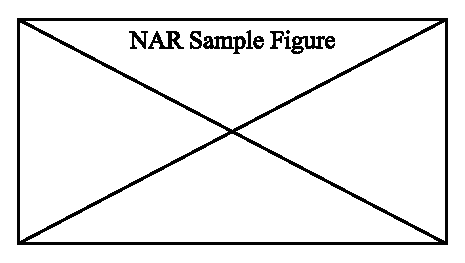
\includegraphics{NAR-fig1.eps}
\end{center}
\caption{Caption for figure within column.}
\label{NAR-fig1}
\end{figure}


\section{RESULTS}

\subsection{The Sesame library}

% !! IMPORTANT !! %
% Say something about the seeds. In particular, it is important to
% mention that we do not do spaced seeds.

We wrote a C library to compute seeding probabilities from the theoretical
results presented in \cite{1}. Briefly, the strategy was to represent
reads and off-target sequences in a custom combinatorial alphabet, specify
the generating functions of basic words and define a language based on a
transfer matrix. The powers of the transfer matrix contain the generating
functions of the reads of interest, from which we can extract their
probability of ocurrence.

The probability that a read contains a seed depends on the problem and on
the read. Sesame computes seeding probabilities from five user-specified
parameters. The problem-specific parameters are known to the user and
consist of the read length $k$, the error rate $p$ and the minimum seed
size $\gamma$. The read-specific parameters are unknown to the user and
consist of the number of duplicates of the target $N$, and their average
sequence divergence $\mu$. We will explain below how to estimate them in
practice.

The Sesame library was built for performance so that it can be integrated
in mapping frameworks. This means that computations are performed only
once for a given set of parameters and memoized for later retrieval. The
parameters $k$, $p$ and $\gamma$ are constant throughout the sequencing
run, but $N$ and $\mu$ must be computed for every read. By default, Sesame
collapses the $(N, \mu)$ pairs to a coarse grid of $15 \times 3=45$
values. Computing all 45 values takes a few minutes on modern hardware,
which is negligible compared to mapping a sequencing run with several
million reads. In addition, the computed values can be saved on disk for
reuse in later runs. The user interface and available options are further
described on the main page of the repository.


\subsection{Comparing seeding strategies}

The seeding step is an essential part of read mapping. Choosing an
appropriate strategy is important, but this is usually based on limited
testing. With accurate seeding probabilities, it is possible to compare
the merits of different seeding strategies, which can be useful for
choosing a seed type or a minimum seed length.

As an example, we compare the default strategies of BWA and Bowtie2 at 1\%
sequencing error. Note that both mappers use advanced methods to refine
the seeding heuristic, so the comparison does not reflect their
performance. It is nevertheless useful to give a baseline for the
potential of each strategy. The default strategy of BWA it to use MEM
seeds of minimum size 19; that of Bowtie2 is to use seeds of size 16 every
ten nucleotides (referred to here as skip-9 seeds).

The worst seeding outcome is that the set of candidate loci contains only
paralogues of target. In this case the target is lost, but worse, the
mapper is on a wrong path and may return a paralogue instead. It is thus
important to control the probability of this outcome referred to as
off-target seeding.

Figure~\ref{fig:mortal_kombat} shows the off-target probabilities computed
by Sesame. Counter-intuitively, the probability initially increases with
the read size for MEM seeds. It turns out that off-target MEM seeds are
common in short reads that contain errors. Since longer reads have a
higher chance of containing an error, the off-target rate initially
increases. This effect dampens so that all the probabilities eventually
decrease exponentially, albeit at different rates.

For skip seeds, the off-target rates decrease in staircase with a drop
every 10 nucleotides. Indeed, the seeds are exactly the same if the read
length stays within the same decade. The curves show an overal linear
trend and have the same asymptotic rate.

From this we draw the important conclusion that the performance of skip
seeds degrades much less than MEM seeds when the target contains
paralogues. Skip seeds are thus better suited for sensitive mapping in
repeated sequences. Incidentally, this Figure~\ref{fig:mortal_kombat}
shows that it is suboptimal for a MEM-based mapper to all the candidate
loci when there is more than a handful of them: if the target has more
than 20 paralogues, the mapping quality will remain low even when the
output is correct. A better strategy is to either bail out or switch to a
more sensitive seeding method (BWA uses a re-seeding policy).

A related observation is that for MEM seeds, the off-target rate is above
$10^{-3}$ for reads of 50 nucleotides or less, meaning that beating
quality 30 is not straightforward in these conditions. It is important to
remember that mapping cannot be wrong if the target has no paralogue
(because it is trivial to recognize that false positives have no homology
with the read). Therefore, the main strategy to reach high mapping
confidence with MEM seeds is not to reduce the minimum seed size, but to
ascertain that the target is a unique sequence. We will show how to do
achieve this below.

Figure~\ref{fig:mortal_kombat} suggests that the performance of skip seeds
is better than that of MEM seeds. However one has to bear in mind that we
compare MEM seeds of size 19 with skip seeds of size 16: the gain in
sensitivity comes at the cost of a larger candidate set. In practice such
a large candidate set must be further filtered (Bowtie2 does this with a
priority policy), so the final performance of skip seeds cannot be as high
as suggested in the figure because of speed constraints.


\section{Estimating $N$ and $\mu$}

Estimating the two read-dependent parameters $N$ and $\mu$ is essential to
compute seeding probabilities. Recall that $N$ is the number paralogues of
the target ($N=0$ means that it is unique) and that $\mu$ is the sequence
divergence (the average fraction of mismatches between a paralogue and the
target).

The key observation is that the seeding algorithm can also reveal the
paralogue structure of the target. Queries in the FM index are carried out
using an algorithm known as the backward search. Extending the query one
nucleotide at a time, the backward search returns the number of matching
sequences in the genome. The decaying number of hits depends on how many
paralogues of the target are present in the genome, and how similar they
are with each other. It is thus possible to use the series of the backward
search to estimate $N$ and $\mu$.

Writing the likelihood of the process is straightforward if we assume that
nucleotides are used uniformly at random in the genome. The difficulty is
that the first iterations of the backward search are uninformative. For
instance, a query of length 10 is expected to have $\geq 3000$ hits in
the genome, so the potential paralogues of the target are hidden among so
many random hits. In practice, we ignore the first iterations until the
number of random hits is lower than 1. The information is labelled as
missing and the likelihood is updated accordingly. This gives a function
that can now by maximized with respect to $N$ and $\mu$.

Initial simulations revealed that the maximum likelihood estimates of $N$
and $\mu$ have a large variance. To mitigate this effect, we opted for a
grid search where we test only plausible values of $\mu$ and compute the
associated $N$ (see Methods). This gave a fast algorithm forced to produce
reasonable estimates.

We initially tested this method on the read, gathering the series of decay
during the seeding process. However, we quickly realized that this method
routinely missed paralogues because of sequencing errors. Using mapping as
an error correction mechanism, we tested a prototype estimating $N$ and
$\mu$ from the sequence of the best hit and obtained significantly better
results, so we settle for this option, even though it is slower. It is of
course possible that the best hit is not the target, but if it is a
paralogue, the estimated values of $N$ and $\mu$ should be similar.

The estimation strategy is depicted in Figure~\ref{fig:strategy}. The
putative target is segmented in windows of 30 nucleotides overlapping by
20 nucleotides. The grid search is run a every window in both the foward
and reverse orientation, ignoring the first 20 iterations of the backward
search. The windowing approach accomodates the fact that only some
regions of the target may be repeated (e.g., if the read straddles a
transposon). Finally, we take the median values of $N$ and $\mu$ as
representative for the whole sequence.


\section{Super reads}

While testing the estimation algorithm on reads of size 50, we observed
that a sub-population of them had mapping error rates below $10^{-5}$.
This is surprising in regard of Figure~\ref{fig:mortal_kombat}a because in
a genome where half of the sequences are duplicated, the error rate should
be $\approx 1/2 10^{-3}$. We reasoned that non-repeated sequences must be
overrepresented in this sub-population of reads.

Those reads are characterized by two facts: $i.$ they have at most one
difference with the best hit and $ii.$ the backward search depicted in
Figure~\ref{fig:strategy} retrived only one sequence on each window.
Individually, these facts are not uncommon in mismapped reads, but
together, they leave little space for error.



\begin{table}[b]
\tableparts{%
\caption{This is a table caption}
\label{table:01}%
}{%
\begin{tabular*}{\columnwidth}{@{}lllll@{}}
\toprule
Col. head 1 & Col. head 2 & Col. head 3 & Col. head 4 & Col. head 5
\\
& (\%) & (s$^{-1}$) & (\%) & (s$^{-1}$)
\\
\colrule
Row 1 & Row 1 & Row 1 & -- & --
\\
Row 2 & Row 2 & Row 2 & Row 2 & Row 2
\\
\botrule
\end{tabular*}%
}
{This is a table footnote}
\end{table}


\subsection{Results subsection two}

Text.  Text. Text. Text. Text. Text. Text. Text. Text. Text. Text.
Text. Text. Text. Text. Text. Text. Text. Text. Text. Text. Text.
Text (see Table \ref{table:01}).

Text. Text. Text. Text. Text. Text.
Text. Text. Text. Text. Text. Text. Text. Text. Text. Text. Text.
Text. Text. Text. Text. Text. Text. Text. Text. Text.
Text (see Figure \ref{NAR-fig2}a).

Text. Text. Text. Text. Text.
Text. Text. Text. Text. Text. Text. Text. Text. Text. Text. Text.
Text. Text. Text. Text. Text. Text. Text. Text. Text. Text. Text.
Text. Text. Text. Text. Text. Text. Text. Text. Text. Text. Text.
Text. Text. Text. Text. Text. Text. Text. Text. Text. Text. Text.
Text. Text. Text. Text. Text. Text. Text. Text. Text. Text. Text.
Text. Text. Text. Text. Text. Text. Text. Text. Text. Text. Text.
Text. Text. Text. Text. Text. Text. Text. Text. Text. Text. Text.
Text. Text. Text. Text. Text. Text. Text. Text. Text. Text. Text.
Text. Text. Text. Text. Text. Text. Text. Text. Text. Text. Text.
Text. Text. Text. Text. Text. Text. Text. Text. Text. Text. Text.
Text. Text. Text. Text. Text. Text. Text. Text. Text. Text.

\begin{figure*}[t]
\begin{center}
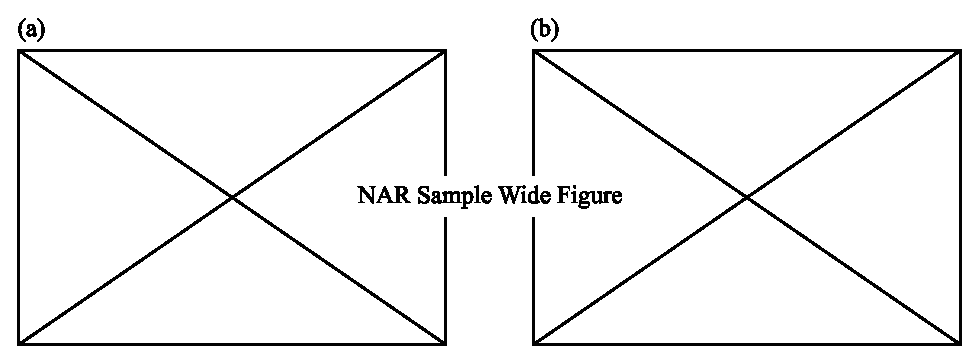
\includegraphics{NAR-fig2.eps}
\end{center}
\caption{Caption for wide figure over two columns.
\textbf{(a)} Left figure.
\textbf{(b)} Right figure (see (a)).
}
\label{NAR-fig2}
\end{figure*}


\subsection{Results subsection three}

Text. Text. Text. Text. Text. Text. Text. Text. Text. Text. Text.
Text. Text. Text. Text. Text. Text. Text. Text. Text. Text. Text.
Text. Text. Text. Text. Text. Text. Text. Text. Text. Text. Text.
Text. Text. Text. Text. Text. Text. Text. Text. Text. Text. Text.
Text. Text. Text. Text. Text. Text. Text. Text. Text. Text. Text.
Text. Text. Text. Text. Text. Text. Text. Text. Text. Text. Text.
Text. Text. Text. Text. Text. Text. Text. Text. Text. Text. Text.
Text. Text. Text. Text. Text. Text. Text. Text. Text. Text. Text.
Text. Text. Text. Text. Text. Text. Text. Text. Text. Text. Text.
Text. Text. Text. Text. Text. Text. Text. Text. Text. Text. Text.
Text. Text. Text.


\section{DISCUSSION}

\subsection{Discussion subsection one}

Text. Text. Text. Text. Text. Text. Text. Text. Text. Text. Text.
Text. Text. Text. Text. Text. Text. Text. Text. Text. Text. Text.
Text. Text. Text. Text. Text. Text. Text. Text. Text. Text. Text.
Text. Text. Text. Text. Text. Text. Text. Text. Text. Text. Text.
Text. Text. Text. Text. Text. Text. Text. Text. Text. Text. Text.
Text. Text. Text. Text. Text. Text. Text. Text. Text. Text. Text.
Text. Text. Text. Text. Text. Text. Text. Text. Text. Text. Text.
Text. Text. Text. Text. Text. Text. Text. Text. Text. Text. Text.
Text. Text. Text. Text. Text. Text. Text. Text. Text. Text. Text.
Text. Text. Text. Text. Text. Text. Text. Text. Text. Text. Text.
Text. Text. Text. Text. Text. Text. Text. Text. Text. Text. Text.
Text. Text. Text. Text. Text. Text. Text. Text. Text. Text. Text.
Text. Text. Text. Text. Text. Text. Text. Text. Text. Text. Text.
Text. Text. Text. Text. Text. Text. Text. Text. Text. Text. Text.
Text. Text. Text. Text. Text. Text. Text. Text. Text. Text. Text.
Text. Text. Text. Text. Text. Text. Text. Text. Text. Text. Text.
Text. Text. Text. Text. Text. Text. Text. Text. Text. Text. Text.
Text. Text. Text. Text. Text. Text. Text. Text. Text. Text. Text.
Text. Text. Text. Text. Text. Text. Text. Text. Text. Text. Text.
Text. Text. Text. Text. Text. Text. Text. Text. Text. Text. Text.
Text. Text. Text. Text. Text. Text.


\subsection{Discussion subsection two}

Text. Text. Text. Text. Text. Text. Text. Text. Text. Text. Text.
Text. Text. Text. Text. Text. Text. Text. Text. Text. Text. Text.
Text. Text. Text. Text. Text. Text. Text. Text. Text. Text. Text.
Text. Text. Text. Text. Text. Text. Text. Text. Text. Text. Text.
Text. Text. Text. Text. Text. Text. Text. Text. Text. Text. Text.
Text. Text. Text. Text. Text. Text. Text. Text. Text. Text. Text.
Text. Text. Text. Text. Text. Text. Text. Text. Text. Text. Text.
Text. Text. Text. Text. Text. Text. Text. Text. Text. Text. Text.
Text. Text. Text. Text. Text. Text. Text. Text. Text. Text. Text.
Text. Text. Text. Text. Text. Text. Text. Text. Text. Text. Text.
Text.

Text. Text. Text. Text. Text. Text. Text. Text. Text. Text. Text.
Text. Text. Text. Text. Text. Text. Text. Text. Text. Text. Text.
Text. Text. Text. Text. Text. Text. Text. Text. Text. Text. Text.
Text. Text. Text. Text. Text. Text. Text. Text. Text. Text. Text.
Text. Text. Text. Text. Text. Text. Text. Text. Text. Text. Text.
Text. Text. Text. Text. Text. Text. Text. Text. Text. Text. Text.
Text. Text. Text. Text. Text. Text. Text. Text. Text. Text. Text.
Text. Text. Text. Text. Text. Text. Text. Text. Text. Text. Text.
Text. Text. Text. Text. Text. Text. Text. Text. Text. Text. Text.
Text. Text. Text. Text. Text. Text. Text. Text. Text. Text. Text.
Text. Text. Text. Text. Text. Text. Text. Text. Text. Text.


\subsection{Discussion subsection three}

Text. Text. Text. Text. Text. Text. Text. Text. Text. Text. Text.
Text. Text. Text. Text. Text. Text. Text. Text. Text. Text. Text.
Text. Text. Text. Text. Text. Text. Text. Text. Text. Text. Text.
Text. Text. Text. Text. Text. Text. Text. Text. Text. Text. Text.
Text. Text. Text. Text. Text. Text. Text. Text. Text. Text. Text.
Text. Text. Text. Text. Text. Text. Text. Text. Text. Text. Text.
Text. Text. Text. Text. Text. Text. Text. Text. Text. Text. Text.
Text. Text. Text. Text. Text. Text. Text. Text. Text. Text. Text.
Text. Text. Text. Text. Text. Text. Text. Text. Text. Text. Text.
Text. Text. Text. Text. Text. Text. Text. Text. Text. Text. Text.
Text. Text. Text. Text. Text. Text. Text. Text. Text.

Text. Text. Text. Text. Text. Text. Text. Text. Text. Text. Text.
Text. Text. Text. Text. Text. Text. Text. Text. Text. Text. Text.
Text. Text. Text. Text. Text. Text. Text. Text. Text. Text. Text.
Text. Text. Text. Text. Text. Text. Text. Text. Text. Text. Text.
Text. Text. Text. Text. Text. Text. Text. Text. Text. Text. Text.
Text. Text. Text. Text. Text. Text. Text. Text. Text. Text. Text.
Text. Text. Text. Text. Text. Text. Text. Text. Text. Text. Text.
Text. Text. Text. Text. Text. Text. Text.

Text. Text. Text. Text. Text. Text. Text. Text. Text. Text. Text.
Text. Text. Text. Text. Text. Text. Text. Text. Text. Text. Text.
Text. Text. Text. Text. Text. Text. Text. Text. Text. Text. Text.
Text. Text. Text. Text. Text. Text. Text. Text. Text. Text. Text.
Text. Text. Text. Text. Text. Text. Text. Text. Text. Text. Text.
Text. Text. Text. Text. Text. Text. Text. Text. Text. Text. Text.
Text. Text. Text. Text. Text. Text. Text. Text. Text. Text. Text.
Text. Text. Text. Text. Text. Text. Text.


\section{CONCLUSION}

Text. Text. Text. Text. Text. Text. Text. Text. Text. Text. Text.
Text. Text. Text. Text. Text. Text. Text. Text. Text. Text. Text.
Text. Text. Text. Text. Text. Text. Text. Text. Text. Text. Text.
Text. Text. Text. Text. Text. Text. Text. Text. Text. Text. Text.
Text. Text. Text. Text. Text. Text. Text. Text. Text. Text. Text.
Text. Text. Text. Text. Text. Text. Text. Text. Text. Text. Text.
Text. Text. Text. Text. Text. Text. Text. Text. Text. Text. Text.
Text. Text. Text. Text. Text. Text. Text. Text. Text. Text. Text.
Text. Text. Text. Text. Text. Text. Text. Text. Text. Text. Text.
Text. Text. Text.


\section{ACKNOWLEDGEMENTS}

Text. Text. Text. Text. Text. Text. Text. Text. Text. Text. Text.
Text. Text. Text. Text.


\subsubsection{Conflict of interest statement.} None declared.
\newpage


\begin{thebibliography}{4}

% Format for article
\bibitem{1}
Author,A.B. and Author,C. (1992)
Article title.
\textit{Abbreviated Journal Name}, \textbf{5}, 300--330.

% Format for book
\bibitem{2}
Author,D., Author,E.F. and Author,G. (1995)
\textit{Book Title}.
Publisher Name, Publisher Address.

% Format for chapter in book
\bibitem{3}
Author,H. and Author,I. (2005)
Chapter title.
In
Editor,A. and Editor,B. (eds),
\textit{Book Title},
Publisher Name, Publisher Address,
pp.\ 60--80.

% Another article
\bibitem{4}
Author,Y. and Author,Z. (2002)
Article title.
\textit{Abbreviated Journal Name}, \textbf{53}, 500--520.

\end{thebibliography}

\end{document}
